\documentclass[12pt]{article}
\usepackage[margin=2.5cm]{geometry}
\usepackage{enumerate}
\usepackage{amsfonts}
\usepackage{amsmath}
\usepackage{fancyhdr}
\usepackage{amsmath}
\usepackage{amssymb}
\usepackage{amsthm}
\usepackage{mdframed}
\usepackage{graphicx}
\usepackage{subcaption}
\usepackage{adjustbox}
\usepackage{listings}
\usepackage{xcolor}
\usepackage{booktabs}
\usepackage[utf]{kotex}

\definecolor{codegreen}{rgb}{0,0.6,0}
\definecolor{codegray}{rgb}{0.5,0.5,0.5}
\definecolor{codepurple}{rgb}{0.58,0,0.82}
\definecolor{backcolour}{rgb}{0.95,0.95,0.92}

\lstdefinestyle{mystyle}{
    backgroundcolor=\color{backcolour},
    commentstyle=\color{codegreen},
    keywordstyle=\color{magenta},
    numberstyle=\tiny\color{codegray},
    stringstyle=\color{codepurple},
    basicstyle=\ttfamily\footnotesize,
    breakatwhitespace=false,
    breaklines=true,
    captionpos=b,
    keepspaces=true,
    numbers=left,
    numbersep=5pt,
    showspaces=false,
    showstringspaces=false,
    showtabs=false,
    tabsize=1
}

\lstset{style=mystyle}

\pagestyle{fancy}
\renewcommand{\headrulewidth}{0.4pt}
\lhead{Hyungmo Gu}
\rhead{CSC209 Week 5 Notes}

\begin{document}
\title{CSC209 Week 5 Notes}
\author{Hyungmo Gu}
\maketitle

\section*{Files in C 1 of 5}

\bigskip

\begin{itemize}
    \item Opening file
    \begin{itemize}
        \item \textbf{Syntax:} *fopen(const char *filename, const char *mode)
        \item the import file should be in the same folder as `a.out' (default)
        \item Mode Strings
        \begin{enumerate}[1.]
            \item \textit{r} - File opened for reading
            \item \textit{w} - File opened for writing
            \item \textit{a} - File opened for appending
        \end{enumerate}

    \begin{lstlisting}[language=c]
    #include <stdio.h>

    int main() {
        FILE *sample_file;

        sample_file = fopen("example_sources/sample.txt", "r");
        if (sample_file == NULL) {
            fprintf(stderr, "Error opening file \n");
            return 1;
        }

        ...

        return 0;
    }
    \end{lstlisting}
    \end{itemize}
    \item Closing file
    \begin{itemize}
        \item \textbf{Syntax:} fclose(FILE *filename)
        \item returns 0 if close successful

    \begin{lstlisting}[language=c]
    #include <stdio.h>

    int main() {
        FILE *sample_file;

        ...

        if (fclose(sample_file) != 0) {
            fprintf(stderr, "fclose failed\n");
            return 1;
        }

        return 0;
    }
    \end{lstlisting}
    \end{itemize}
\end{itemize}

\bigskip

\section*{Files in C 2 of 5}

\bigskip

\begin{itemize}
    \item Reading from Files
    \begin{itemize}
        \item \textbf{Syntax:} char *fgets(char *s, int n, FILE *stream)
        \item Reads data line by line
        \begin{enumerate}[1.]
            \item \textit{char *s} is a pointer to memory where text can be stored
            \begin{itemize}
                \item Note new var can be created here, like for loop (i.e. for(i=0; i < 1; i++)).
                \item On success, fgets returns \textit{s}
                \item On failure, fgets returns NULL
            \end{itemize}
            \item \textit{int n} is the maximum upper number of characters fgets allowed to put in \textit{s}
        \end{enumerate}
    \end{itemize}

    \begin{lstlisting}[language=c]
    #include <stdio.h>

    #define LINE_LENGTH 80

    int main() {
        FILE *sample_file;
        int error;
        char line[LINE_LENGTH + 1];

        sample_file = fopen("example_sources/sample.txt", "r");

        while (fgets(line, LINE_LENGTH + 1, sample_file) != NULL) {
            printf("%s", line);
        }

        ...
        return 0;
    }
    \end{lstlisting}

    \item Reading from Input
    \begin{itemize}
        \item \textbf{Syntax:} fgets(line, LINE\_LENGTH + 1, stdin)
        \item Notice \textit{stdin} is the standard input, like input in Python
    \end{itemize}
    \begin{lstlisting}[language=c]
    #include <stdio.h>

    #define LINE_LENGTH 80

    int main() {
        char line[LINE_LENGTH + 1];

        while (fgets(line, LINE_LENGTH + 1, stdin) != NULL) {
            printf("%s", line);
        }

        return 0;
    }
    \end{lstlisting}
\end{itemize}

\bigskip

\section*{Files in C 3 of 5}

\bigskip

\begin{itemize}
    \item The scanf function
    \begin{itemize}
        \item returns successfully read items
        \item number of read items depends on format
        \item \textbf{Syntax:} int fscanf(FILE *stream, const char *format, type *s,  type *n)
    \end{itemize}

    \begin{lstlisting}[language=c]
    #include <stdio.h>

    #define LINE_LENGTH 80

    int main() {
        FILE *sample_file;
        int error, score, total;

        sample_file = fopen("example_sources/sample.txt", "r");
        if (sample_file == NULL) {
            perror("Error opening file\n");
            return 1;
        }

        while (fscanf(sample_file, "%d %d", &score, &total) == 2) { //<- ==2 means each fscan must return 2 values, one for each col.
            printf("Score: %d, Total: %d.\n", score, total);
        }

        error = fclose(sample_file);
        if (error != 0) {
            perror("fclose failed on input file\n");
            return 1;
        }

        return 0;
    }
    \end{lstlisting}
\end{itemize}

\bigskip

\section*{Files in C 4 of 5}

\bigskip

\begin{itemize}
    \item Writing to Files
    \begin{itemize}
        \item \textbf{Syntax:} output\_file = fopen(const char *filename, "w")
        \begin{itemize}
            \item \textit{w} overwrites existing file
            \item \textit{a} appends output to the end of file
        \end{itemize}

        \begin{lstlisting}[language=c]
        #include <stdio.h>

        int main() {
            FILE *output_file;
            int error;
            int total = 50;
            float small_number = 0.125;

            output_file = fopen("example_sources/output.txt", "w");
            if (output_file == NULL) {
                perror("Error opening file\n");
                return 1;
            }

            fprintf(output_file, "The first line in the file\n");
            fprintf(output_file, "The integer is %d\n", total);
            fprintf(output_file, "The small float is %f\n", small_number);

            ...

            return 0;
        }
        \end{lstlisting}

        \item NOTE: the output stream is first stored in memory controlled by OS
        before to disk

        \begin{center}
        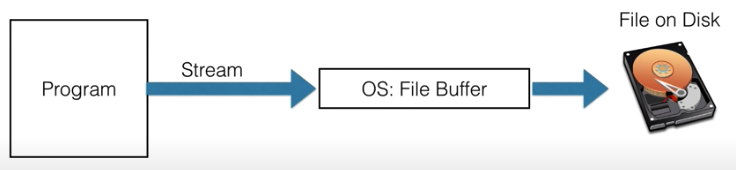
\includegraphics[width=\linewidth]{images/week_5_notes_part_4_1.png}
        \end{center}

        \begin{itemize}
            \item OS periodically writes content from memory to disk
            \item Abnormal computer shutdown $\to$ some data may be lost
        \end{itemize}
    \end{itemize}

    \begin{lstlisting}[language=c]

    \end{lstlisting}
\end{itemize}

\bigskip

\section*{Files in C 5 of 5}

\bigskip

\begin{itemize}
    \item Bringing Everything Together

    \begin{lstlisting}[language=c,caption={files\_example\_5.c}]
    #include <stdio.h>

    int main() {
        FILE *sample_file, *output_file;
        int error_open, error_closed, score;
        int total = 50;

        sample_file = fopen("example_sources/sample.txt", "r");
        if (sample_file == NULL) {
            fprintf(stderr, "Error opening file \n");
            return 1;
        }

        output_file = fopen("example_sources/output.txt", "w");
        if (output_file == NULL) {
            perror("Error opening file\n");
            return 1;
        }

        while (fscanf(sample_file, "%d %d", &score, &total) == 2) {
            printf("Score: %d\n", score);
            fprintf(output_file, "Score: %d\n", score);
        }

        error_open = fclose(sample_file);
        if (error_open != 0) {
            perror("fclose failed\n");
            return 1;
        }

        error_closed = fclose(output_file);
        if (error_closed != 0) {
            perror("fclose failed\n");
            return 1;
        }

        return 0;
    }
    \end{lstlisting}

\end{itemize}

\bigskip

\section*{Strings in C 1 of 6}

\bigskip

\begin{itemize}
    \item Introduction to Strings
    \begin{itemize}
        \item String is an array of chars with `$\backslash0$' at the end
        \begin{itemize}
            \item i.e. `hello' = [`h',`e',`l',`l',`o',`$\backslash0$']
            \item without `$\backslash0$', undesired output is included, i.e. hello?[BT

    \end{itemize}
    \end{itemize}
\end{itemize}

\end{document}